% siminos/spatiotemp/chapter/action.tex
% $Author: predrag $ $Date: 2021-12-24 01:25:20 -0500 (Fri, 24 Dec 2021) $

% \ifblog  Predrag 2021-06-12 gave up on this,
%          do not remember who calls it other than blogCats.tex
    \chapter{Hill's formula}
    \label{c-Hill}  % temporary, while being edited in spatiotemp/
%\renewcommand{\cl}[1]{{\ensuremath{n_{#1}}}}   % discrete length of a cycle, Predrag
\renewcommand{\shift}{\ensuremath{\ell}}

\section{An overview over ``Hill's formulas''}
\label{sect:Hill}
%\renewcommand{\cl}[1]{{\ensuremath{|#1|}}}  % the length of a periodic orbit, Ronnie
\renewcommand{\shift}{\ensuremath{d}}

\begin{quote}
A succinct  explanation of the Hill's formula:\\
If you evaluate stability of the 3-term recurrence \refeq{JiKoKr20(2)} on
a periodic lattice you get the {\jacobianOrb} $\jMorb$;
if you evaluate it by multiplying the `two-configuration representation'
matrix $\jMps$, you get the `time evolution' side of the Hill's formula.
\end{quote}

We should emphasize that, while discovered first in Lagrangian setting,
Hill's formulas are much more general, they
apply also to dissipative dynamical systems as well, see

CL18 \HREF{http://chaosbook.org/~predrag/papers/CL18.pdf\#subsection.1.5}
{sect.~1.5} {\em  Stability of an orbit vs.  its time-evolution stability}

CL18 \HREF{http://chaosbook.org/~predrag/papers/CL18.pdf\#appendix.C}
{appendix~C} {\em Spatiotemporal stability}


\refsect{LiTom17b:GenFctn} {\em Generating functions; action}
%\else  Predrag 2021-06-12 gave up on this,
%          do not remember who calls it other than blogCats.tex
%\subsection{Generating functions; action}
%\fi


\refsect{sect:HillLagr} {\em Hill's formula, Lagrangian setting}


\refsect{sect:catlattHill} {\em \catLatt\ Hill's formula}


\refsect{sect:catlattHillrel} {\em Hill's formula for \rpo s}


\refsect{sect:templattHillHan} {\em Han's \templatt\ Hill's formula}


\refsect{sect:catlattHillHan} {\em Han's  \catlatt\ Hill's formula}


\refsect{sect:catlattHillRelativeHan} {\em Han's relative-periodic Hill's formula}


\refsect{sect:HenonHillHan} {\em Han's  \HenonMap\ Hill's formula}











\section{Generating functions; action}
%\else  Predrag 2021-06-12 gave up on this,
%          do not remember who calls it other than blogCats.tex
%\subsection{Generating functions; action}
%\fi
\label{LiTom17b:GenFctn}

    \PC{2016-11-11, 2018-09-26}{
What follows is (initially)
copied from Li and Tomsovic\rf{LiTom17b}, \emph{Exact relations between
homoclinic and \po\ actions in chaotic systems} arXiv source
file, then merged with the MacKay-Meiss-Percival action
principle \refrefs{MKMP84,meiss92}.
    }
For discrete-time one-degree-of-freedom Lagrangian systems satisfying a
periodicity condition (\ie, cat map):
\beq
\genF(\coord+1, \coord'+1)=\genF(\coord, \coord')+C
\,,
\ee{MacMei83-2}
one can consider relative periodic paths (or pre-periodic paths, also called
periodic paths of type $(\shift,\cl{})$ by Mackay and Meiss\rf{MacMei83}), with
    \PC{2018-09-29} {presumably they are \rpo s, or pre-\po s, with a rational
    winding number $p/\coord$.}
\beq
\coord_{i+\cl{}}=\coord_{i}+\shift
\,.
\ee{MacMei83-3}
Every $\coord_{i}$ returns to its value after time period $\cl{}$, but shifted by
$\shift$.
Orbits satisfying \refeq{MacMei83-3} are given by stationary points of the action
\beq
\action = \sum_{i=0}^{q-1} \genF(\coord_i, \coord_{i+1})
\ee{MacMei83-4}
in the space of periodic paths of type $(\shift,\cl{})$.
For periodic paths, it suffices to consider one period, because an orbit is periodic if
and only if it is a stationary point of the action of one period in the space
of periodic paths.

If the constant $C$ (the
\HREF{https://floerhomology.wordpress.com/2015/09/14/mean-action-and-the-calabi-invariant/}
{Calabi invariant}\rf{Calabi70}) in the periodicity condition
\refeq{MacMei83-2} is zero, and the Lagrangian satisfies a convexity
condition
\beq
\genF_{12}(\coord, \coord') < 0
\,,
\ee{MacMei83-5}
where subscript $k$ refers to the derivative with respect to the $k$th
argument, then the action of periodic paths of type  $(\shift,\cl{})$ is bounded below,
so there is a minimising path. Since its action is stationary, it gives a \po\
of type  $(\shift,\cl{})$.

    \PC{2018-01-21}{Is this true?
To go from the Hamiltonian $(\ssp_{\zeit},p_{\zeit})$ phase space formulation to the
Newtonian (or Lagrangian) $(\ssp_{\zeit-1},\ssp_{\zeit})$ {\em state space}
formulation, replace $p_\zeit$  by
\(
p_\zeit = (\ssp_{\zeit} - \ssp_{\zeit-1})/\Delta\zeit \,,
\)
where $\Delta\zeit =1$.
    }
    %
For {\orbit} ${p}$  of period $\cl{p}$, the {action} of the \orbit\ is:
\beq
\label{eq:DefGenFprimePOs}
\action_{p}  \equiv \sum_{n=0}^{\cl{p}-1}\genF(\coord_{n},\coord_{n+1})\ .
\eeq
$\action_{p}$ is the generating function that maps a point along the orbit for one
(prime) period.  For the case of a fixed point $p$ of period $\cl{p}=1$,
the action is
\beq\label{eq:Definition generating function fixed points}
\action_{p}  = \genF(\coord_p,\coord_p)
\,,
\eeq
where the generating function $\genF(\coord_p,\coord_p)$ maps $\ssp_p$ into itself in one
iteration.

\section{Homoclinic and \po\ actions in chaotic systems}

    \PC{2018-09-29}{
What follows is copied from Li and Tomsovic\rf{LiTom17b}.
    }
For an aperiodic orbit $\lbrace\ssp_0\rbrace$ going through the point $\ssp_0$,
the action, evaluated as the sum over an infinity of successive mappings,
\begin{equation}
\label{eq:full orbit action in general}
\action_{\lbrace \ssp_0 \rbrace}
\equiv \lim_{N \to \infty}
\sum_{n=-N}^{N-1} \genF(\coord_{n},\coord_{n+1})
=\lim_{N \to \infty} \action_{-N,N}
\,,
\end{equation}
is not necessarily convergent. However, the MacKay-Meiss-Percival action
principle\rf{MKMP84,meiss92} can be applied to obtain well defined
action differences between pairs of orbits.  For example,
the {\em relative} {\em action}
$\Delta \action_{\lbrace h_0 \rbrace  \lbrace x \rbrace}$ between a fixed point $\ssp_p$
and its homoclinic orbit $\lbrace h_{0} \rbrace$, where $h_{\pm
\infty}\to \ssp_p$:
\begin{eqnarray}
\label{eq:relative action homoclinic}
\Delta \action_{\lbrace h_0 \rbrace  \lbrace \ssp_p \rbrace}
 &\equiv & \lim_{N \to \infty} \sum_{i=-N}^{N-1}\left[\genF(h_i,h_{i+1})-\genF(\ssp_p,\ssp_p)\right]
\nonumber \\
&=& \int\limits_{U[\ssp_p,h_{0}]}p\mathrm{d}\coord+\int\limits_{S[h_{0},\ssp_p]}p\mathrm{d}\coord
= \oint_{US[\ssp_p,h_{0}]} p\mathrm{d}\coord \nonumber \\
&=& {\cal A}^\circ_{US[\ssp_p,h_{0}]}
\end{eqnarray}
where $U[\ssp_p,h_{0}]$ is the segment of the unstable manifold from $\ssp_p$ to
$h_{0}$, and $S[h_{0},\ssp_p]$ the segment of the stable manifold from $h_0$
to $\ssp_p$.  The $\circ$ superscript on the last line indicates that the area
is interior to a path that forms a closed loop, and the subscript
indicates the path: $US[\ssp_p,h_{0}]=U[\ssp_p,h_{0}]+S[h_{0},\ssp_p]$.  The
clockwise enclosure of an area is positive, counterclockwise negative.
$\Delta \action_{\lbrace h_0 \rbrace \lbrace \ssp_p \rbrace} $ gives the
action difference between the homoclinic orbit segment $[
h_{-N},\cdots,h_{N} ]$ and the length-$(2N+1)$ fixed point orbit segment
$[ \ssp_p, \cdots, \ssp_p ]$ in the limit $N \to \infty$. In later sections, upon
specifying the symbolic code of the homoclinic orbit $\lbrace h_0 \rbrace
\Rightarrow \overline{0} \gamma \overline{0}$, we also denote $\Delta
\action_{\lbrace h_0 \rbrace  \lbrace \ssp_p \rbrace}$ alternatively as
\begin{equation}\label{eq:relative action homoclinic symbolic notation}
\Delta \action_{\lbrace h_0 \rbrace  \lbrace \ssp_p \rbrace}
= \Delta \action_{\overline{0} \gamma \overline{0},  \overline{0}}
\end{equation}
by replacing the orbits in the subscript with their symbolic codes.

%%%%%%%%%%%%%%%%%%%%%%%%%%%%%%%%%%%%%%%%%%%%%%%%%%%%%%%%%%%%%%%%%%%%%
\begin{figure}
   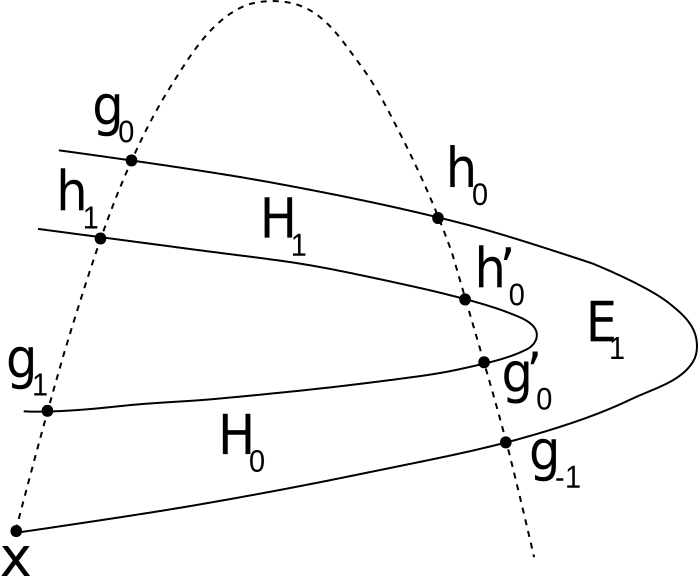
\includegraphics[width=0.5\textwidth]{LiTom17bHorseshoe2}
\caption{\label{fig:Horseshoe2}
A sketch of a partial homoclinic tangle
which forms a complete horseshoe structure. The unstable (stable)
manifold of $x$ is the solid (dashed) curve. There are two primary
homoclinic orbits $\lbrace h_0\rbrace$ and $\lbrace g_0\rbrace$.
$\cal{R}$ is the closed region bounded by loop
$\mathcal{L}_{USUS[x,g_{-1},h_0,g_0]}$.
~(From \refref{LiTom17b})
        }
\end{figure}
%%%%%%%%%%%%%%%%%%%%%%%%%%%%%%%%%%%%%%%%%%%%%%%%%%%%%%%%%%%%%%%%%%%%%

Likewise, a second important case is for the relative action between a
pair of homoclinic orbits $\lbrace h^{\prime}_0\rbrace \Rightarrow
\overline{0} \gamma^{\prime} \overline{0} $ and $\lbrace h_0\rbrace
\Rightarrow \overline{0} \gamma \overline{0}$, which results in
\begin{eqnarray}
\label{eq:homoclinic action difference}
\Delta \action_{{\lbrace h^{\prime}_0\rbrace}{\lbrace h_0\rbrace}} &\equiv & \lim_{N \to \infty} \sum_{i=-N}^{N-1}\left[ \genF(h^{\prime}_{i},h^{\prime}_{i+1}) - \genF(h_{i},h_{i+1})\right] \nonumber \\
& = & \lim_{N \to \infty} \left[ \genF(h^{\prime}_{-N},h^{\prime}_{N}) - \genF(h_{-N},h_{N}) \right] \nonumber \\
& = & \int\limits_{U[h_{0},h^\prime_{0}]}p\mathrm{d}\coord+\int\limits_{S[h^\prime_{0},h_{0}]}p\mathrm{d}\coord =  {\cal A}^\circ_{US[h_0,h^\prime_{0}]} \nonumber \\
& = & \Delta \action_{ \overline{0} \gamma^{\prime} \overline{0},  \overline{0} \gamma \overline{0} }
\end{eqnarray}
where $U[h_{0},h^\prime_{0}]$ is the segment of the unstable manifold
from $h_{0}$ to $h^\prime_{0}$, and $S[h^\prime_{0},h_{0}]$ the segment
of the stable manifold from $h^\prime_{0}$ to $h_{0}$.  Due to the fact
that the endpoints approach $\ssp_p$ forward and backward in time, one can
also write
\begin{eqnarray}
\label{eq:homoclinic action difference2}
\Delta \action_{{\lbrace h^{\prime}_0\rbrace}{\lbrace h_0\rbrace}}
& = & \lim_{N \to \infty}
\left[ \genF(h^{\prime}_{-(N+n)},h^{\prime}_{N+m}) - \genF(h_{-N},h_{N})
      \right] \nonumber \\
& & - (n+m) {\cal F}_0
\,.
\end{eqnarray}

%%%%%%%%%%%%%%%%%%%%%%%%%%%%%%%%%%%%%%%%%%%%%%%%
    \ifblog
\newpage
% siminos/spatiotemp/chapter/Hill.tex
% $Author: predrag $ $Date: 2021-12-08 23:33:01 -0500 (Wed, 08 Dec 2021) $

%\chapter{Hill's formula} %called by blogCats.tex and CL18.tex
%\label{c-Hill}  % temporary, while being edited in spatiotemp/

%\Chapter{Hill}{28jan2018}{Hill's formula}   % formatted for ChaosBook.org
%\label{c-Hill}
%\listofsections{0}

\section{Hill's formula, Lagrangian setting}
\label{sect:HillLagr}

    \PC{2016-11-11, 2018-09-26}{
The current draft of this section starts out with
excerpts from
Mackay and Meiss\rf{MacMei83}
{\em Linear stability of periodic orbits in {Lagrangian} systems},
 and
Bolotin and Treschev\rf{BolTre10} {\em Hill's formula}.
    }
%
There can be more than one minimising path. In particular,
translating one minimising path by an integer in time or space or both gives
another. This implies existence of saddle points of the action in between the
minima, with one downward direction [1-3]. They are called minimax points, and
give rise to minimax \po s of type $(\shift,\cl{})$. The statement of the existence of
at least two \po s of each type  $(\shift,\cl{})$ is known as the Poincar\'e-Birkhoff
theorem.

As a corollary, Mackay and Meiss\rf{MacMei83} rederive the old result
that when the convexity condition is satisfied, the multipliers of a
minimising orbit are a reciprocal pair of positive reals, and those of a
minimax orbit are either a complex conjugate pair on the unit circle, or
a reciprocal pair of negative reals. The result for minimising orbits was
shown by \Poincare\rf{Poinc1886} for two-degree-of-freedom
continuous-time systems, and Birkhoff [1] discusses the minimax case.

The linear stability of a \po\ is determined by its multipliers, the eigenvalues
of the derivative of the return map round the orbit. While the first variation of
the action is by definition zero for an orbit, the multipliers of a \po\ can be
related to the second variations of the action in the space of periodic paths.
This has been shown in various cases. Hill\rf{Hill86} and \Poincare\rf{Poinc1886}
derived a formula for the multipliers in the case of one-degree-of-freedom
systems of the form kinetic minus potential\rf{Hill86}, using a Fourier
representation for periodic paths. In his study of \po s of the three-body
problem, Hill obtained a formula connecting the characteristic polynomial of the
monodromy matrix of a \po\ with the infinite determinant of the Hessian of the
action functional. Mackay and Meiss\rf{MacMei83} derived a formula
\refeq{MacMei83(17)} for the multipliers of a \po\ for general discrete-time
one-degree-of-freedom systems. Bolotin and Treschev\rf{BolTre10} give two
multidimensional generalizations of Hill's formula: for discrete Lagrangian
systems (symplectic twist maps) and for continuous Lagrangian systems, and
discuss implications of symmetries and reversibility. Bountis and
Helleman\rf{Bount81} and Greene\rf{gree79} treated the case of discrete-time
one-degree-of-freedom systems with
\beq
\genF_{12}(\coord,\coord') = -1
\,.
\ee{MacMei83(6)}
Schmidt\rf{Schmidt84} determined $n$-tupling bifurcations by the criterion
that the matrix of second variations of the action
with respect to periodic paths of $n$ times the period
have a zero eigenvalue.


Mackay and Meiss\rf{MacMei83} relate the multipliers of a periodic orbit to the second variations of
the action about the orbit, and compute the {\HillDet} of the matrix
of second variations of the action in the space of periodic
paths of period $\period{}$.

Stationarity \refeq{MKMP84(3.7)} of the action for an orbit of a
discrete-time one-degree-of-freedom system implies that
\beq
\genF_2(\coord_{i-1},\coord_{i}) + \genF_1(\coord_i,\coord_{i+1}) = 0
\,.
\ee{MacMei83(7)}
Thus the tangent orbits $\delta \ssp_i$ satisfy [...]. The multipliers
\ExpaEig\ of a \po\ of period $q$ are
defined by existence of a tangent orbit satisfying [...] residue of a \po\
one can easily solve for multipliers. [... losing steam]


Mackay and Meiss\rf{MacMei83} formulas for the multipliers of minimising and
minimax orbits follow. Under the convexity condition
\refeq{MacMei83-5}, the denominator is positive. At a minimum of action
(whether local or global):
\beq
D(1) \leq 0
\,,
\ee{MacMei83-18}
so the multipliers are real and positive. At a minimax with one downward
direction:
\beq
D(1) \geq 0
\,,
\ee{MacMei83-19}
so the multipliers are on the unit circle or the negative real axis.

Residue\rf{gree79} $R$ of a \po\ $p$ of period \cl{p}
\beq
4R = \det(\matId-\jMps_p)
   = \tr(\matId-\jMps_p)
   = 2-\ExpaEig_p-1/\ExpaEig_p
\ee{MacMei83(16)}
is related to the {\HillDet} $D(\ExpaEig)$ by
what the discrete Hill's formula\rf{BolTre10}:
    \PC{2018-09-30}{See Bolotin and Treschev\rf{BolTre10} eqs.~(2.8) and (2.13)}
\beq
\det (\matId-\jMps_p) = -D(1)\left(\prod_{i=0}^{\cl{p}-1}(-\genF_{12}[i,i+1])\right)^{-1}
\,.
\ee{MacMei83(17)}
This formula was derived by Mackay and Meiss\rf{MacMei83} and
Allroth\rf{Allroth83} (Allroth eq.~(12)). It applies to general
``one-degree-of-freedom'' systems, \ie, 1D lattices with only the nearest
neighbor interactions. For a finite set of neighbors, \ie, higher\dmn\
discrete-time systems, Allroth\rf{Allroth83} has some partial results in the
context of Frenkel-Kontorova models.

$D(1)$ is the {\HillDet} of the matrix of second variations of
the action in the space of periodic paths of period q. So we have related the
multipliers of a \po\ to the second variations of the action about
the orbit.

\newpage %TEMP
\renewcommand\speriod[1]{{\ensuremath{L_{#1}}}}  %continuous spatial period
\renewcommand\period[1]{{\ensuremath{T_{#1}}}}  %continuous time period
%
\section{\catLatt\ Hill's formula}
\label{sect:catlattHill}

\begin{description}
  \item[2020-07-23 Predrag]
I have everything in place for deriving \catlatt\ (and \templatt as a special
case) Hill's formula from the elementary Kronecker product
\refeq{KroneckerProd} block matrix rules
    \begin{enumerate}
      \item multiplication \refeq{mixedProd} leads to
            shift \refeq{shiftPower} accruing correctly.
      \item {\HillDet} \refeq{wikiKron2}, \refeq{detShiftxJ};
            yields correct ln det = tr ln reduction to periodic $J_p$
      \item $\mathbf{A}\otimes\mathbf{B}$ being similar to
            $\mathbf{B}\otimes\mathbf{A}$ by \refeq{wikiKron3} explains why
            [$2\speriod{}\!\times\!2\speriod{}$] phase space is
            equivalent to the [$\speriod{}\!\times\!\speriod{}$] orbit
            stability.
    \end{enumerate}
  \item[2020-07-23 Predrag]
Next: streamline, move to CL18.tex
  \item[2020-07-27 Predrag]
Essential parts copied to CL18.tex, \emph{siminos/kittens/Hill.tex}
\end{description}

\bigskip\bigskip

The $d=2$ lattice \catlatt\ equations can be recast in a
matrix form, by rewriting the defining equations as block
matrices\rf{Dorr70,ChenM87,HuRyCo98}, constructed by the
\HREF{https://en.wikipedia.org/wiki/Kronecker_product} {Kronecker
product} $\mathbf{A}\otimes\mathbf{B}$,%
    \PC{2020-08-01}{The Zehfuss product (1858), really. The {\HillDet} is
    from 1886, though it does not look recognizably anything like out the
    {\HillDet}s... These things are
    \HREF{https://www.cs.cornell.edu/cv/ResearchPDF/KPHist.pdf}
    {everywhere!}
    }
an operation that replaces
elements of the [$n\times{n}$] matrix $\mathbf{A}$ by [$m\times{m}$]
matrix `blocks' $\mathbf{B}$, resulting in an [$mn\times mn$] block
matrix\rf{ArWeHa13,wikiKronProd}
\beq
\mathbf{A}\otimes\mathbf{B} =
\left[\begin{array}{ccc} %\begin{bmatrix}
  a_{11} \mathbf{B} & \cdots & a_{1n}\mathbf{B} \\
             \vdots & \ddots &           \vdots \\
  a_{n1} \mathbf{B} & \cdots & a_{nn} \mathbf{B}
\end{array}\right] %\end{bmatrix}
\,.
\ee{KroneckerProd}
Consider $\mathbf{A}$, $\mathbf{C}$ square matrices of size
[$n\times{n}$], and $\mathbf{B}$, $\mathbf{D}$ square matrices of size
[$m\times{m}$].
The matrix product of two block matrices is a block
matrix\rf{ArWeHa13,wikiBlockMat},
\beq
(\mathbf{A}\otimes\mathbf{B})\,(\mathbf{C}\otimes\mathbf{D})
%= (\mathbf{A}\mathbf{C})\otimes(\mathbf{B}\mathbf{D})
%  {\displaystyle (\mathbf {A} \otimes \mathbf {B} )(\mathbf {C} \otimes \mathbf {D} )
  =(\mathbf{AC})\otimes (\mathbf{BD})
  \,.
\ee{mixedProd}
The trace and the determinant of a block matrix are given by
\bea
\tr(\mathbf {A} \otimes \mathbf {B})
    &=& \tr\mathbf{A}\,\tr\mathbf{B}
    \continue
\det\left(\mathbf{A} \otimes \mathbf{B}\right)
    &=& \det\left(\mathbf{A}^{m}\right) \det\left(\mathbf{B}^{n}\right)
\,.
\label{wikiKron2}
\eea
The two [$mn\times mn$] block matrices $\mathbf{A}\otimes\mathbf{B}$ and
$\mathbf{B}\otimes\mathbf{A}$ are equivalent by a similarity
transformation
\beq
\mathbf {B} \otimes \mathbf {A}
=\transp{\mathbf {P}} \,(\mathbf {A} \otimes \mathbf {B} )\,\mathbf {P}
\,,
\ee{wikiKron3}
where $\mathbf{P}$ is permutation matrix. As $\det{\mathbf{P}}=1$,
the block matrix determinant
$\det\left(\mathbf{A}\otimes\mathbf{B}\right)
=
\det\left(\mathbf{B}\otimes\mathbf{A}\right)$
is independent of the order in which blocks are constructed.

Now, apply this formalism to a $\BravCell{\speriod{}}{\period{}}{0}$ rectangular Bravais
cell. In the Kronecker product block matrix notation
\refeq{KroneckerProd}, the \jacobianOrb\ refeq\{eq:BxAtempJ\} can be
written as a $[\speriod{}\period{}\times\speriod{}\period{}]$ block
matrix
\beq
\jMorb
=
\unit_{1} \otimes \left(\shift_{2}+\shift_{2}^{-1}\right)
-
2 {s}\,\unit_1\otimes\unit_{2}
+
\left(\shift_{1}+\shift_{1}^{-1}\right) \otimes \unit_{2}
\,,
\ee{catalattLxT}
where the \refeq{KroneckerProd} matrix $\mathbf{A}$ and identity
$\unit_1$ matrix are `spatial' [$\speriod{}\!\times\!\speriod{}$]
matrices, with blocks $\mathbf{B}$ and identity $\unit_2$ `temporal'
[$\period{}\!\times\!\period{}$] matrices, with indices `1', `2'
referring to `spatial', `temporal' lattice directions, respectively.

Our goal is to compute the {\HillDet} $|\det \jMorb|$. As we have
shown in the example refsect\{s:catLattRel3x2\},  % a CL18.tex section
this is best done directly, by computing the volume of the {\fundPip}.
    \PC{2020-07-27}{
Insert refsect\{s:catLattRel3x2\} example here?
    }

However, in classical and statistical mechanics, one often computes the
{\HillDet} using a  Hamiltonian, or `transfer matrix' formulation.
An example is the \templatt\ 3-term recurrence
\refeq{genFuncts:CatMapNewt} % in the blog
%\refeq{eq:CatMapNewt} % in CL18.tex
in the \PV\rf{PerViv} `two-configuration' cat map representation
\refeq{eq:StateSpCatMap}
%     \PC{2020-07-15}{in CL18 remove \refeq{eq:StateSpCatMap_Hill}}
\beq
 \hat{\mathbf{\ssp}}_{\zeit+1} =
      {\hat{\mathbf{\jMps}}_1}\,\hat{\mathbf{\ssp}}_\zeit - \hat{\mathsf{\Ssym{}}}_\zeit
\,,
\ee{PV2config}
with the one-time step temporal evolution [$2\!\times\!2$] {\jacobian}
matrix ${\hat{\mathbf{\jMps}}_1}$ generating a time orbit by acting on the
2\dmn\ `phase space' of successive configuration points
\beq
 {\hat{\mathbf{\jMps}}_1}
=
 \left[\begin{array}{cc}
 0 & 1 \\
 -1 & s
 \end{array} \right]
\,,\qquad
\hat{\mathbf{\ssp}}_\zeit
=
\left(
\begin{array}{c}
 \ssp_{\zeit-1}\\
 \ssp_{\zeit}
 \end{array}
 \right)
\,,\qquad
\hat{\mathsf{\Ssym{}}}_\zeit
=
    \left(
\begin{array}{c}
 0           \\
 \Ssym{\zeit}
 \end{array}
    \right)
\,,
\ee{PV2configJ}
Similarly, for the $d=2$ \catlatt\ lattice at hand, one can
recast the 5-term recurrence (XX) %\refeq{CatMap2d}
(compare with the \refeq{FGHLW74:charFunct1d})
\bea
\ssp_{n\zeit}
&=& ~~\ssp_{n\zeit}
%(- \ssp_{n+1,\zeit-1} + 2{s} \, \ssp_{n,\zeit-1} - \ssp_{n-1,\zeit-1})
%- \Ssym{n,\zeit-1}
%- \ssp_{n,\zeit-2}
    \continue
\ssp_{n,\zeit+1}
&=&  - \ssp_{n,\zeit-1}
 +(- \ssp_{n-1,\zeit} + 2{s} \, \ssp_{n\zeit} - \ssp_{n+1,\zeit})
- \Ssym{n\zeit}
%\,,
\label{CatMap2dHill}
\eea
in the `two-configuration' matrix form \refeq{PV2config} by picking the
vertical direction (indexed `2') as the `time', with temporal 1-time step {\jacobian}
[$2\speriod{}\!\times\!2\speriod{}$] block matrix
% ${\hat{\mathbf{\jMps}}_1}$
\beq
{\hat{\mathbf{\jMps}}_1}  =
 \left[\begin{array}{c|c}
{\bf 0} & \unit_1\\ \hline
-\unit_1 & {-\mathbf{\jMorb}_1}
 \end{array} \right]
\,,
\ee{PV2catlattJ}
(known as a transfer matrix in statistical
mechanics\rf{Onsager44,MonMun94}) generating a time orbit by acting on a
$2\speriod{}$\dmn\ `phase space'  lattice strip
$\hat{\mathbf{\ssp}}_\zeit$ along the `spatial' direction  (indexed `1'),
\beq
\hat{\mathbf{\ssp}}_\zeit
=
\left[\begin{array}{c}
 {\mathbf{\ssp}}_{\zeit-1}\\ \hline
 {\mathbf{\ssp}}_\zeit
 \end{array}\right]
,\quad
\hat{\mathsf{\Ssym{}}}_\zeit
=
    \left[\begin{array}{c}
    \mathbf{0}\\ \hline
 \mathbf{\Ssym{}}_{1\zeit}
 \end{array}\right]
,\qquad
\mathbf{\ssp}_\zeit
=
\left[\begin{array}{c}
 \ssp_{1\zeit}\\   \vdots\\ \ssp_{\speriod{}\zeit}
 \end{array}\right]
,\quad
\mathsf{\Ssym{}}_\zeit
=
    \left[\begin{array}{c}
 \Ssym{1\zeit}\\ \vdots\\ \Ssym{\speriod{}\zeit}
 \end{array}\right]
,
\ee{PV2catlattJ1}
where the hat $\hat{~}$~ indicates a $2\speriod{}$\dmn\
`two-configuration' state, and $\mathbf{\jMorb}_1$ is the spatial
$[\speriod{}\!\times\!\speriod{}]$ {\jacobianOrb} of  form (XX),
\beq
\mathbf{\jMorb}_1
        =
\shift_{1}^{-1} - 2s \unit_1 + \shift_{1}
\label{Hessian_Hill}
\eeq
The `two-configuration' coupled cat maps system \refeq{PV2config} is a
generalization of the Bernoulli map time evolution formulation (XX) to a
higher-dimensional spatially-coupled lattice.
Just as in the {temporal Bernoulli} condition refeq \{tempFixPoint\}, the
first order in time difference equation \refeq{PV2config} can be viewed
as a {\lattstate} fixed point condition refeq\{tempFixPoint\}, a
zeros of the function
\( %beq
F[\hat{\Xx}] = \hat{\mathbf{\jMorb}}\hat{\Xx}+\hat{\Mm} = 0
\,,
\) %\ee{tempPV2Point}
with the entire periodic \emph{{\lattstate}} $\hat{\Xx}_{\Mm}$ treated as a
single fixed \emph{point} in the
$2\speriod{}\period{}$\dmn\ unit hyper-cube, and the
$[2\speriod{}\period{}\times2\speriod{}\period{}]$  block matrix \jacobianOrb\
given either by
\beq
\hat{\mathbf{\jMorb}} =
    \hat{\unit} - {\hat{\mathbf{\jMps}}_1}\otimes\shift_2^{-1}
\,,
\ee{tempPV2conf12}
or by
\beq
\hat{\mathbf{\jMorb}}' =
    \hat{\unit} -\shift_2^{-1} \otimes {\hat{\mathbf{\jMps}}_1}
\,.
\ee{tempPV2conf21}
Here the unity $\hat{\unit}=\hat{\unit}_1\otimes\unit_{2}$ is a
[$2\speriod{}\period{}\!\times\!2\speriod{}\period{}$] block matrix, and
the time-evolution \jacobianM\ ${\hat{\mathbf{\jMps}}_1}$
\refeq{PV2catlattJ} is a [$2\speriod{}\!\times\!2\speriod{}$] matrix.

The order in which the block matrix blocks are composed does not matter,
yielding the same the {\HillDet} $\det\hat{\mathbf{\jMorb}} =
\det\hat{\mathbf{\jMorb}}'$ by \refeq{wikiKron3}.
However, written out explicitly, the two \jacobianOrbs\
\refeq{eq:orbitJPVJxS} and \refeq{eq:orbitJPVtempJ} are of a very
different form.

For example, for the $\BravCell{\speriod{}}{\period{}}{0}$  rectangular
Bravais cell, the \catlatt\ \jacobianOrb\ (XX) involves the
[$\period{}\!\times\!\period{}$] time {\shiftOp} block matrix $\shift_2$
(XX) with the one-time-step [$2\speriod{}\!\times\!2\speriod{}$]
time-evolution \jacobianM\ ${\hat{\mathbf{\jMps}}_1}$ \refeq{PV2catlattJ}
\bea
\hat{\mathbf{\jMorb}}
    &=&
\left[\begin{array}{c|c}
 \unit_{1}\otimes\unit_{2}   & -\unit_1\otimes\shift_2^{-1}             \\ \hline
 \unit_1\otimes\shift_2^{-1}& \unit_{1}\otimes\unit_{2} +\mathbf{\jMorb}_1\otimes\shift_2^{-1}
\end{array}\right]
\,,
\label{eq:orbitJPVJxS}
\eea
and for \catlatt\ \refeq{CatMap2dHill} this is a time-periodic
[$\period{}\times\period{}$]  {\shiftOp} block matrix $\shift_2$ (XX),
each block now a space-periodic [$2\speriod{}\!\times\!2\speriod{}$] matrix
${\hat{\mathbf{\jMps}}_1}$ \refeq{PV2catlattJ}.

If a block matrix is composed of four blocks,
\HREF{https://en.wikipedia.org/wiki/Block_matrix\#Block_matrix_inversion}
{its determinant} can be factorized by Schur's (1917)
formula\rf{Schur1917,wikiBlockMat}
    \index{Schur!formula}
% \refeq{det2x2blockMat***
\beq
\det\left[\begin{array}{c|c}
\mathbf{A} & \mathbf{B} \\ \hline
\mathbf{C} & \mathbf{D}
\end{array}\right]
=
\det(\mathbf{A})\,\det(\mathbf{D}-\mathbf{C}\mathbf{A}^{-1}\mathbf{B})
\,.
\ee{det2x2blockMat}
so, noting \refeq{mixedProd}, \refeq{catalattLxT} and
\refeq{Hessian_Hill}, we find that the
$[2\speriod{}\period{}\times2\speriod{}\period{}]$ `phase space'
$\det\hat{\mathbf{\jMorb}}$ defined by \refeq{eq:orbitJPVJxS} is actually
the desired {\HillDet} of
$[\speriod{}\period{}\times\speriod{}\period{}]$ \jacobianOrb\
$\mathbf{\jMorb}$,
\bea
\det\hat{\mathbf{\jMorb}}
    &=&
\det\left[\begin{array}{c|c}
 \unit_{1}\otimes\unit_{2}   & -\unit_1\otimes\shift_2^{-1}             \\ \hline
 \unit_1\otimes\shift_2^{-1}& \unit_{1}\otimes\unit_{2} +\mathbf{\jMorb}_1\otimes\shift_2^{-1}
\end{array}\right]
     \continue
     &=&
% \det(\unit_1)\,
\det\left[
       \unit_{1}\otimes\unit_{2} + \mathbf{\jMorb}_1\otimes\shift_2^{-1}
     + (\unit_1\otimes\shift_2^{-1})(\unit_{1}\otimes\unit_{2})(\unit_1\otimes\shift_2^{-1})
    \right]
     \continue
     &=&
\det\left[
       \unit_{1}\otimes\unit_{2} + \mathbf{\jMorb}_1\otimes\shift_2^{-1}
     +  \unit_1\otimes\shift_2^{-2}
    \right]
     \continue
     &=&
\det(\shift_2^{-1})\,
\det\left[
       \unit_1\otimes\shift_2^{-1}
        +(\shift_{1}^{-1} - 2s \unit_1 + \shift_{1})\otimes\unit_2
     +  \unit_1\otimes\shift_2
    \right]
     \continue
     &=&
\det \jMorb
\,,
\label{det2x2blockMat2LH}
\eea
where we have used
$\det\unit_{1}=\det\unit_{2}=\det\shift_{1}=\det\shift_{2}=1$.

Consider next \refeq{tempPV2conf21}, the equivalent way of forming of the
block matrix for the $\BravCell{\speriod{}}{\period{}}{0}$  rectangular
Bravais cell, with temporal period taken for definitiveness $\period{}=4$.
The \catlatt\ \jacobianOrb\ \refeq{tempPV2conf21} is now constructed as
the [$4\times4$] time {\shiftOp} block matrix $\shift_2$ (XX), with the
one-time-step [$2\speriod{}\!\times\!2\speriod{}$] time-evolution
\jacobianM\ ${\hat{\mathbf{\jMps}}_1}$ \refeq{PV2catlattJ} and unit
matrix $\hat{\unit}_1$ as blocks
\beq
\hat{\mathbf{\jMorb}}'
 =
\unit_2\otimes\hat{\unit}_{1} -\shift_2^{-1} \otimes {\hat{\mathbf{\jMps}}_1}
 =
\left[\begin{array}{c|c|c|c}
 \hat{\unit}_1    &  {\bf 0}   & {\bf 0}    &-{\hat{\mathbf{\jMps}}_1} \\ \hline
-{\hat{\mathbf{\jMps}}_1} &  \hat{\unit}_1   & {\bf 0}    & {\bf 0}    \\ \hline
 {\bf 0}    &-{\hat{\mathbf{\jMps}}_1} & \hat{\unit}_1    & {\bf 0}    \\ \hline
 {\bf 0}    &  {\bf 0}   &-{\hat{\mathbf{\jMps}}_1} & \hat{\unit}_1
\end{array}\right]
\,.
\label{eq:orbitJPVtempJ}
\eeq
To evaluate the {\HillDet} $\det\hat{\mathbf{\jMorb}}'$, note that from
the block-matrix multiplication rule \refeq{mixedProd} and the determinant rule \refeq{wikiKron2}
it follows that
\beq
(\shift_2^{-1}\otimes{\hat{\mathbf{\jMps}}_1})
(\shift_2^{-1}\otimes{\hat{\mathbf{\jMps}}_1})
=
\shift_2^{-2}\otimes{\hat{\mathbf{\jMps}}_1}^2
\,,\quad
(\shift_2^{-1} \otimes {\hat{\mathbf{\jMps}}_1})^k =
\shift_2^{-k} \otimes {\hat{\mathbf{\jMps}}_1}^k
\,,
\ee{shiftPower}
and
\beq
\det(\shift_2^{-1}\otimes{{\hat{\mathbf{\jMps}}_1}})
=
(\det\shift_2)^{-\speriod{}}
(\det{\hat{\mathbf{\jMps}}_1})^\period{}
=
\det\hat{\mathbf{\jMps}}_p
\,,\qquad
\hat{\mathbf{\jMps}}_p = {\hat{\mathbf{\jMps}}_1}^\period{}
\,,
\ee{detShiftxJ}
where $\hat{\mathbf{\jMps}}_p$ is the {\jacobianM} of a
temporal periodic orbit $p$.
Expand
\(
 \ln\det\hat{\mathbf{\jMorb}}'
   =
 \tr\ln\hat{\mathbf{\jMorb}}'
\)
as a series using \refeq{wikiKron2} and \refeq{shiftPower},
\beq
\tr\ln\hat{\mathbf{\jMorb}}' =
\tr\ln(\unit-\shift_2^{-1} \otimes {{\hat{\mathbf{\jMps}}_1}})
  =
-\sum_{k=1}^\infty\frac{1}{k}{\tr(\shift_2^{-k})}\,\tr{{\hat{\mathbf{\jMps}}_1}}^{k}
\,,
\ee{LnDet=TrLn_Hill}
and use
$\Tr \shift_2^k=\period{}$
if $k$ is a multiple of $\period{}$,
0 otherwise
(follows from $\shift_2^\period{}=\unit$):
\[
\ln\det(\unit-\shift_2^{-1} \otimes {{\hat{\mathbf{\jMps}}_1}})
  =
-\sum_{r=1}^\infty\frac{1}{r}\tr\hat{\mathbf{\jMps}}_p^{r}
  =
\ln\det(\hat{\unit}_{1}-\hat{\mathbf{\jMps}}_p)
\,.
\]
So for the {\catlatt} the {\jacobianOrb}  and the temporal evolution
\refeq{PV2config} stability ${{\hat{\mathbf{\jMps}}_{p}}}$ are related by
the remarkable Hill's formula
\beq
|\det\jMorb|
  =
|\det(\hat{\unit}_{1}-\hat{\mathbf{\jMps}}_p)|
\,.
\ee{detBern2n}
which expresses the  {\HillDet} of the arbitrarily large \jacobianOrb\
$\hat{\mathbf{\jMorb}}'$  in terms of a determinant of a small
[$2\speriod{}\!\times\!2\speriod{}$] time-evolution \jacobianM\
${\hat{\mathbf{\jMps}}_1}$.

{\bf Remark}                                \toCB
From \refeq{det2x2blockMat1} we have
\beq
\det {\hat{\mathbf{\jMps}}_1} =
\det
 \left[\begin{array}{cc}
{\bf 0} & \unit_1\\
-\unit_1 & {-\mathbf{\jMorb}_1 }
\end{array}
\right]
=
\det(\mathbf{\jMorb}_1)\,\det(\mathbf{\jMorb}_1^{-1}) = 1
\,,
\ee{det2x2blockMat3}
so ${\hat{\mathbf{\jMps}}_1}$ is a canonical, or phase-space volume preserving
transformation, as one expects of Hamiltonian systems.


{\bf Remark}
The reformulation of the \catlatt\ 5-term recurrence \refeq{CatMap2dHill}
as the `two-configuration' form \refeq{PV2config} is really just the
usual passage from Lagrangian to the Hamiltonian formulation, but we
chose to short-circuit it, as all that heavy general formalism is not
needed for the problem at hand.
    \PC{2020-07-15}{
Perhaps refer to \toChaosBook{section.8.1} {8.1 Hamiltonian flows}.
Mention transfer matrix formulation of lattice field theories?
    }

{\bf Remark}
I am not a big fan of the Kronecker product \refeq{KroneckerProd} as it
treats the time and the space differently. Nicer notion would be a tensor
product that treats all directions in $d$\dmn\ on equal, symmetric
footing. Perhaps the `outer product' does that (see the
\HREF{https://en.wikipedia.org/wiki/Outer_product} {wiki})  explains the
outer product of tensors, and its relation to the  Kronecker product.
Arfken, Weber \& Harris\rf{ArWeHa13}
{\em Mathematical Methods for Physicists: A Comprehensive Guide}
 \CBlibrary{ArWeHa13} call it
the \emph{direct tensor} or \emph{Kronecker} product, see
\HREF{http://chaosbook.org/library/ArWeHa13chap2.pdf\#section*.29}
{AWH eq.~(2.55)}.
    \index{Kronecker!product}\index{direct tensor!product}

Perhaps Steeb and Hardy\rf{SteHar11} {\em Matrix Calculus, Kronecker
Product and Tensor Product} (I have not downloaded the book) deals with
that. Not sure if that is different from
Steeb and Hardy\rf{SteHar11a} {\em Matrix Calculus and Kronecker Product
- A Practical Approach to Linear and Multilinear Algebra}.

Kowalski and Steeb\rf{KowSte91}
{\em Nonlinear Dynamical Systems and Carleman Linearization}
\CBlibrary{KowSte91} already
goes beyond the other Kronecker product references I had looked at,
as it emphasizes commutators of Kronecker products.

Horn and Johnson\rf{HoJo90} {\em Matrix Analysis} \CBlibrary{HoJo90}
promises to do Kronecker product in the companion volume Horn and
Johnson{HoJo94} {\em Topics in Matrix Analysis} that I have not looked
yet.

Schur's (1917) formula \refeq{det2x2blockMat} is derived in exercise~A.12
of Stone and Goldbart{StGo09} {\em Mathematics for Physics}
\CBlibrary{StGoAppA}.

\section{Hill's formula for \rpo s}
\label{sect:catlattHillrel}

As a first try, let's reverse-engineer relative periodicity for the more
familiar `two-configuration' \catlatt\ \refeq{PV2config}. The stability
matrix of a temporally {\po}
\beq
 \delta\hat{\mathbf{\ssp}}_{\period{}} =
      {\hat{\mathbf{\jMps}}_1^\period{}}\,\delta\hat{\mathbf{\ssp}}_0
\,,
\ee{PV2configPO}
corresponds {\spt}ly to a $\BravCell{\speriod{}}{\period{}}{0}$
rectangular Bravais cell, while the stability matrix of a {\rpo} includes
the relative shift \tilt{},
\beq
 \delta\hat{\mathbf{\ssp}}_{\period{}} = \shift_{1}^\tilt{}
      {\hat{\mathbf{\jMps}}_1^\period{}}\,\delta\hat{\mathbf{\ssp}}_0
\,,
\ee{PV2configRPO}
and corresponds {\spt}ly to a
$\BravCell{\speriod{}}{\period{}}{\tilt{}}$ parallelepipedal Bravais
cell, which can be convert into a rectangular cell by going into a
co-moving frame, with the temporal 1-time step {\jacobian}
[$2\speriod{}\!\times\!2\speriod{}$] block matrix \refeq{PV2catlattJ}
replaced by
\beq
\tilde{\mathbf{\jMps}}_1
  \Rightarrow
      \shift_{1}^{\tilt{}/\period{}}
      \hat{\mathbf{\jMps}}_1
  =
 \left[\begin{array}{c|c}
{\bf 0} & \shift_{1}^{\tilt{}/\period{}}\\ \hline
-\shift_{1}^{\tilt{}/\period{}} &
     {-\shift_{1}^{\tilt{}/\period{}}\mathbf{\jMorb}_1}
 \end{array} \right]
\,,
\ee{PV2catlattJrpo}
and
\(
\hat{\mathbf{\jMorb}}'_{\BravCell{\speriod{}}{\period{}}{\tilt{}}}
\)
is of the rectangular cell form, with replacement
$\hat{\mathbf{\jMps}}_1\to\tilde{\mathbf{\jMps}}_1$ in
\refeq{eq:orbitJPVtempJ}. In evaluating the corresponding determinants we
can use \refeq{detShiftxJ},
\beq
\det(\shift_2^{-1}\otimes{{\tilde{\mathbf{\jMps}}_1}})
=
(\det\shift_2)^{-\speriod{}}
(\det{\tilde{\mathbf{\jMps}}_1})^\period{}
=
\det\tilde{\mathbf{\jMps}}_p
\,,\qquad
\tilde{\mathbf{\jMps}}_p =
      \shift_{1}^{\tilt{}}
      \hat{\mathbf{\jMps}}_1^\period{}
\,,
\ee{detShiftxJrpo}
where $\tilde{\mathbf{\jMps}}_p$ is the {\jacobianM} of the temporal
prime \rpo\ $p$.

Now we can reverse-engineer relative periodicity for the $d=2$ lattice.
We have just worked out $\hat{\mathbf{\jMorb}}'$ defined by
\refeq{tempPV2conf21}.
Consider next $\hat{\mathbf{\jMorb}}$ \refeq{tempPV2conf12},
with `time' and `space' blocked in the other order,
defined by \refeq{tempPV2conf12}, \refeq{eq:orbitJPVJxS} and
\refeq{PV2catlattJrpo},
\bea
\hat{\mathbf{\jMorb}}
    &=&
\left[\begin{array}{c|c}
 \unit_{1}\otimes\unit_{2}   & -\shift_{1}^{\tilt{}/\period{}}\otimes\shift_2^{-1}             \\ \hline
 \shift_{1}^{\tilt{}/\period{}}\otimes\shift_2^{-1} &
      \unit_{1}\otimes\unit_{2} +\mathbf{\jMorb}_1\shift_{1}^{\tilt{}/\period{}}\otimes\shift_2^{-1}
\end{array}\right]
\,,
\label{eq:orbitJPVJxSrpo}
\eea
We next evaluate
the
$[2\speriod{}\period{}\times2\speriod{}\period{}]$ `phase space'
$\det\hat{\mathbf{\jMorb}}$ defined by \refeq{eq:orbitJPVJxS},
and show again that it equals
the {\HillDet} of
$[\speriod{}\period{}\times\speriod{}\period{}]$ \jacobianOrb\
$\mathbf{\jMorb}$,
\bea
\det\hat{\mathbf{\jMorb}}
     &=&
\det\left[
       \unit_{1}\otimes\unit_{2}
     + \mathbf{\jMorb}_1\shift_{1}^{\tilt{}/\period{}}\otimes\shift_2^{-1}
     +  \shift_{1}^{2\tilt{}/\period{}}\otimes\shift_2^{-2}
    \right]
     \continue
     &=&
\det\left[
       \shift_{1}^{\tilt{}/\period{}}\otimes\shift_2^{-1}
        +(\shift_{1}^{-1} - 2s \unit_1 + \shift_{1})\otimes\unit_2
     +  \shift_{1}^{-\tilt{}/\period{}}\otimes\shift_2
    \right]
     \continue
     &=&
\det \jMorb
\,,
\label{det2x2blockMat2rpo}
\eea
The \jacobianOrb\ \refeq{catalattLxT} for a tilted Bravais domain
(\rpo) is thus a
$[\speriod{}\period{}\times\speriod{}\period{}]$ block matrix
\beq
\jMorb_{\BravCell{\speriod{}}{\period{}}{\tilt{}}}
=
\left(\shift_{1}^{\tilt{}/\period{}}\otimes\shift_2^{-1}
      +\shift_{1}^{-\tilt{}/\period{}}\otimes\shift_2\right)
-
2 {s}\,\unit_1\otimes\unit_{2}
+
\left(\shift_{1}+\shift_{1}^{-1}\right) \otimes \unit_{2}
\,.
\ee{catalattLxTrop}
All the relative periodicity is in the
$\shift_{1}^{-\tilt{}/\period{}}\otimes\shift_2$. This space-time
asymmetry is a consequence of choosing the Hermite normal form
\refeq{Holmin12-Hermite} to define the Bravais cell, so we are not home
yet - even though we are computing the representation-independent
determinants, we do not have an invariant statement of cell's `tilt'.

What do I mean? An example of an invariant condition is the statement that
a prime lattice $\lattice_p$ tiles the given lattice $\lattice$ only if
the area spanned by the two `tilted' basis vectors
\beq
\mathbf{a}_2\times\mathbf{a}^p_{2}=\tilt{}\period{p}-\period{}\tilt{p}
\ee{primeTiling}
is a multiple of the prime tile
area $\speriod{p}\period{p}$.




\bigskip\bigskip
{\bf Remark}
Perhaps we can use Floquet theory analogue of a comoving frame
\refeq{PV2catlattJrpo} to put the generally time-varying
$(\hat{\mathbf{\jMps}}_{1})_{\zeit}$ into an average, constant per time
step form $\tilde{\mathbf{\jMps}}_1$, in order to use the block-matrix
formalism.


\section{Han's \templatt\ Hill's formula}
\label{sect:templattHillHan}

The \jacobianOrb\ of the $\period{}=4$ \templatt\ has form:
\[
\jMorb
=
\left(
\begin{array}{cccc}
 -s & 1 & 0 & 1 \\
 1 & -s & 1 & 0 \\
 0 & 1 & -s & 1 \\
 1 & 0 & 1 & -s \\
\end{array}
\right)
\,.
\]

For example, the $\period{}=4$  the \jacobianOrb\ expressed in the terms
of the one-step [$2\times2$] temporal \jacobianM\
\refeq{PV2config} is:
\bea
{\hat{\mathbf{\jMps}}_1}=\unit- \shift^{-1} \otimes \jMps
    \label{eq:orbitJPVtempJHL}\\ %\continue
    &=&
%{\hat{\mathbf{\jMps}}_1}=\unit- \shift^{-1} \otimes \jMps =
\left(
\begin{array}{cc|cc|cc|cc}
 1 & 0 & 0 & 0 & 0 & 0 & 0 & -1 \\
 0 & 1 & 0 & 0 & 0 & 0 & 1 & -s \\ \hline
 0 & -1 & 1 & 0 & 0 & 0 & 0 & 0 \\
 1 & -s & 0 & 1 & 0 & 0 & 0 & 0 \\ \hline
 0 & 0 & 0 & -1 & 1 & 0 & 0 & 0 \\
 0 & 0 & 1 & -s & 0 & 1 & 0 & 0 \\ \hline
 0 & 0 & 0 & 0 & 0 & -1 & 1 & 0 \\
 0 & 0 & 0 & 0 & 1 & -s & 0 & 1 \\
\end{array}
\right)
\,.
\nnu
\eea

\[
\det \left( \unit- \shift^{-1} \otimes \jMps \right)
=
\det \left( \unit-\jMps \otimes \shift^{-1} \right)
=
\det \left[\left( \unit-\jMps \otimes \shift^{-1} \right) \left( \unit_{[2\times 2]} \otimes \shift \right)\right]
\, ,
\]
where:
\[
\unit-\jMps \otimes \shift^{-1}
=
\left(
\begin{array}{cccc|cccc}
 1 & 0 & 0 & 0 & 0 & 0 & 0 & -1 \\
 0 & 1 & 0 & 0 & -1 & 0 & 0 & 0 \\
 0 & 0 & 1 & 0 & 0 & -1 & 0 & 0 \\
 0 & 0 & 0 & 1 & 0 & 0 & -1 & 0 \\ \hline
 0 & 0 & 0 & 1 & 1 & 0 & 0 & -s \\
 1 & 0 & 0 & 0 & -s & 1 & 0 & 0 \\
 0 & 1 & 0 & 0 & 0 & -s & 1 & 0 \\
 0 & 0 & 1 & 0 & 0 & 0 & -s & 1 \\
\end{array}
\right)
\, ,
\]
and
\[
\left( \unit-\jMps \otimes \shift^{-1} \right) \left( \unit_{[2\times 2]} \otimes \shift \right)
=
\left(
\begin{array}{cccc|cccc}
 0 & 1 & 0 & 0 & -1 & 0 & 0 & 0 \\
 0 & 0 & 1 & 0 & 0 & -1 & 0 & 0 \\
 0 & 0 & 0 & 1 & 0 & 0 & -1 & 0 \\
 1 & 0 & 0 & 0 & 0 & 0 & 0 & -1 \\ \hline
 1 & 0 & 0 & 0 & -s & 1 & 0 & 0 \\
 0 & 1 & 0 & 0 & 0 & -s & 1 & 0 \\
 0 & 0 & 1 & 0 & 0 & 0 & -s & 1 \\
 0 & 0 & 0 & 1 & 1 & 0 & 0 & -s \\
\end{array}
\right)
\,.
\]
A block matrix is a matrix defined by smaller matrices, called blocks.
The determinant of a block matrix is\rf{wikiBlockMat}
(see \HREF{https://en.wikipedia.org/wiki/Block_matrix\#Block_matrix_inversion}
{wiki}):
\beq
\det
\left(
\begin{array}{cc}
A & B \\
C & D \\
\end{array}
\right)
=
\det(A)\,\det(D-CA^{-1}B)
\,.
\ee{det2x2blockMat4}
or
\beq
\det
\left(
\begin{array}{cc}
A & B \\
C & D \\
\end{array}
\right)
=
\det(D)\,\det(A-BD^{-1}C)
\,.
\ee{det2x2blockMat4LH}

\section{Han's  \catlatt\ Hill's formula}
\label{sect:catlattHillHan}

Consider a $\BravCell{\speriod{}}{\period{}}{0}$ rectangular Bravais
cell. In the Kronecker product block matrix notation
\refeq{KroneckerProd}, the \jacobianOrb\  refeq\{eq:BxAtempJ\} is the
$[\speriod{}\period{}\times\speriod{}\period{}]$ block matrix
\refeq{catalattLxT}:
\[
\jMorb
=
\unit_{1} \otimes \left(\shift_{2}+\shift_{2}^{-1}\right)
-
2 s \unit%_{[\speriod{}\period{}\times\speriod{}\period{}]}
+
\left(\shift_{1}+\shift_{1}^{-1}\right) \otimes \unit_{2}
\,.
\]
The temporal {\jacobian} matrix $\mathbf{\jMps}$ is:
\[
\mathbf{\jMps} =
 \left(
 \begin{array}{cc}
{\bf 0}_{1} & \unit_{1}\\
-\unit_{1} & {-\hat{\mathbf{\jMorb}}_{1}}
 \end{array}
 \right) \, ,
\]
where $\hat{\mathbf{\jMorb}}_{1}$ is a $[\speriod{}\times\speriod{}]$ matrix
\refeq{Hessian_Hill}:
\[
\hat{\mathbf{\jMorb}}_{1}
=
\shift^{-1}_{1} - 2s \unit_{1} + \shift_{1}
\,.
\]
There is another $[2\speriod{}\period{}\times2\speriod{}\period{}]$
\jacobianOrb:
\[
\jMorb'
=
\unit%_{[2\speriod{}\period{}\times2\speriod{}\period{}]}
- \shift^{-1}_{2} \otimes \mathbf{\jMorb}_1
\,.
\]
Here we will show that:
\[
\det \jMorb = \det \jMorb'
\,.
\]
\bea
\det \jMorb'
&=&
\det \left(
\unit%_{[2\speriod{}\period{}\times2\speriod{}\period{}]}
- \shift^{-1}_{2} \otimes \mathbf{\jMorb}_1
\right)
=
\det \left(
\unit%_{[2\speriod{}\period{}\times2\speriod{}\period{}]}
- \mathbf{\jMorb}_1
\otimes \shift^{-1}_{2}
\right) \continue
&=&
\det \left[
\left(
\unit%_{[2\speriod{}\times2\speriod{}]}
\otimes
\shift_{2}
\right)
\left(
\unit%_{[2\speriod{}\period{}\times2\speriod{}\period{}]}
- \mathbf{\jMorb}_1
\otimes \shift^{-1}_{2}
\right)
\right] \continue
&=&
\det \left(
\unit%_{[2\speriod{}\times2\speriod{}]}
\otimes
\shift_{2}
-
\mathbf{\jMorb}_1
\otimes \unit_{2}
\right) \continue
&=&
\det \Big\{
 \left(
 \begin{array}{cc}
\unit_{1}\otimes\shift_{2}
&
0\\
0
&
\unit_{1}\otimes\shift_{2}
 \end{array}
 \right)
 -
  \left(
 \begin{array}{cc}
0
&
\unit_{1}\otimes\unit_{2}
\\
-\unit_{1}\otimes\unit_{2}
&
-\hat{\mathbf{\jMorb}}_{1}
\otimes
\unit_{2}
 \end{array}
 \right)
\Big\}
\continue
&=&
\det
  \left(
 \begin{array}{cc}
\unit_{1}\otimes\shift_{2}
&
-\unit_{1}\otimes\unit_{2}
\\
\unit_{1}\otimes\unit_{2}
&
\unit_{1}\otimes\shift_{2}
+\hat{\mathbf{\jMorb}}_{1}\otimes\unit_{2}
 \end{array}
 \right)
\continue
&=&
\det \left(
\unit_{1}\otimes\shift_{2}
+\hat{\mathbf{\jMorb}}_{1}\otimes\unit_{2}
+\unit_{1}\otimes\shift^{-1}_{2} \right)
\continue
&=&
\det \jMorb
\, .
\eea

\subsection{Han's relative-periodic Hill's formula}
\label{sect:catlattHillRelativeHan}

Consider a `tilted' or `relative periodic'
$\BravCell{\speriod{}}{\period{}}{S}$ Bravais cell for which we have
after one time period:
\[
\hat{\mathbf{\jMps}}_p \hat{\mathbf{u}}_\zeit
= \hat{\mathbf{u}}_{\zeit+\period{}}
=
%\left[\begin{array}{c|c}
%\shift_1^{S} & 0 \\ \hline
%0 & \shift_1^{S}
%\end{array}\right]
% \hat{\mathbf{u}}_\zeit
% =
\mathbf{\LieEl}_\tilt{}^{-1} \hat{\mathbf{u}}_\zeit
 \,,
\]
so
\[
    \left(
\hat{\unit}_{1} - \mathbf{\LieEl}_\tilt{}\hat{\mathbf{\jMps}}_p
    \right)\hat{\mathbf{u}}_\zeit = 0
\,.
\]


First we will show that:
\bea
\det \hat{\mathbf{\jMorb}}' = \det \left(\hat{\unit}_{1}
   - \mathbf{\LieEl}_\tilt{} \hat{\mathbf{\jMps}}_p \right) \, ,
\label{RelativeHill}
\eea
where
\beq
\mathbf{\LieEl}_\tilt{} =
\left[\begin{array}{c|c}
\shift_1^{S} & 0 \\ \hline
0 & \shift_1^{S}
\end{array}\right]
\,,
\ee{tiltHL}
The right hand side of \refeq{RelativeHill} is different from
\refeq{detBern2n}, because ...

Note that $\mathbf{\LieEl}_\tilt{}$ and $\hat{\mathbf{\jMps}}_1$ commute.
Let $u_{n\zeit}$ be a variation on the field $\ssp_{n\zeit}$.
\[
\hat{\mathbf{u}}_\zeit
=
\left[\begin{array}{c}
 {\mathbf{u}}_{\zeit-1}\\ \hline
 {\mathbf{u}}_\zeit
 \end{array}\right]
 ,\qquad
\mathbf{u}_\zeit
=
\left[\begin{array}{c}
 u_{1\zeit}\\   \vdots\\ u_{\speriod{}\zeit}
 \end{array}\right] \,.
\]
Now we need to know the form of $\hat{\mathbf{\jMorb}}'$ in \refeq{RelativeHill}. Let:
\[
\hat{\mathbf{u}} =
\left[\begin{array}{c}
 \hat{\mathbf{u}}_{1} \\ \hline
 \hat{\mathbf{u}}_{2}\\ \hline
 \vdots \\ \hline
 \hat{\mathbf{u}}_{\period{}-1} \\ \hline
 \hat{\mathbf{u}}_{\period{}}
 \end{array}\right] \, .
\]
Then
\[
\hat{\mathbf{\jMorb}}' =
\left[\begin{array}{cccc}
 \hat{\unit}_1    &   &     &-{\hat{\mathbf{\jMps}}_1} \mathbf{\LieEl}_\tilt{} \\
-{\hat{\mathbf{\jMps}}_1} &  \hat{\unit}_1   & &  \\
     &  & \ddots    &     \\
     &  &-{\hat{\mathbf{\jMps}}_1} & \hat{\unit}_1
\end{array}\right] \, ,
\]
where $\mathbf{\LieEl}_\tilt{}$ is the `tilt' \refeq{tiltHL}, and
$\hat{\mathbf{\jMorb}}' \hat{\mathbf{u}} = 0$ for a periodic perturbation
field. In an analogy with the usual construction of Floquet matrices, let
$\mathbf{\LieEl}^{1/\period{}}_\tilt{}$ be a $\period{}$'th root of the total
relative shift $\mathbf{\LieEl}_\tilt{}$.
Change the field to a co-moving frame
$\hat{\mathbf{u}}_\zeit \to \hat{\mathbf{w}}_\zeit$,
where
\(
\hat{\mathbf{u}}_\zeit
=\mathbf{\LieEl}^{-\zeit/\period{}}_\tilt{}\hat{\mathbf{w}}_\zeit
\,.
\)
Now $\hat{\mathbf{\jMorb}}'$ is replaced by
$\hat{\mathbf{\jMorb}}_{\tilt{}}'$:
\[
\hat{\mathbf{\jMorb}}_{\tilt{}}' =
\hat{\unit}-\shift_2^{-1} \otimes
       \left(
\hat{\mathbf{\jMps}}_1\mathbf{\LieEl}^{1/\period{}}_\tilt{}
       \right)
\,.
\]
Then we have $\hat{\mathbf{\jMorb}}_{\tilt{}}' \hat{\mathbf{w}} = 0$
when $\hat{\mathbf{\jMorb}}' \hat{\mathbf{u}} = 0$. Using the method from
\refeq{LnDet=TrLn_Hill},
\[
\det \hat{\mathbf{\jMorb}}_{\tilt{}}'
= \det \left[ \hat{\unit}_{1} -
            \left(
\hat{\mathbf{\jMps}}_1\mathbf{\LieEl}^{1/\period{}}_\tilt{}
            \right)^{\period{}}
        \right]
=  \det \left( \hat{\unit}_{1} - {\hat{\mathbf{\jMps}}_1}^{\period{}} \mathbf{\LieEl}_\tilt{} \right)
=  \det \left( \hat{\unit}_{1} - \mathbf{\LieEl}_\tilt{} {\hat{\mathbf{\jMps}}_1}^{\period{}} \right)
\, .
\]

When we change to the co-moving frame $\hat{\mathbf{u}}_\zeit \to \hat{\mathbf{w}}_\zeit$, all of the operators are changed by a similarity transformation:
\[
\hat{\mathbf{\jMorb}}_{\tilt{}}' =
\hat{\mathbf{P}} \hat{\mathbf{\jMorb}}' \hat{\mathbf{P}}^{-1} \, ,
\]
where
\[
\hat{\mathbf{P}} = \text{diag} \left(
\mathbf{\LieEl}^{1/\period{}}_\tilt{},
\mathbf{\LieEl}^{2/\period{}}_\tilt{},
\dots,
\mathbf{\LieEl}^{(\period{}-1)/\period{}}_\tilt{},
\mathbf{\LieEl}_\tilt{}
\right)
\]
is a $[2\speriod{}\period{}\times2\speriod{}\period{}]$ block diagonal matrix. In the co-moving frame, we have
\(
\hat{\mathbf{w}}_\zeit
= \mathbf{\LieEl}^{\zeit/\period{}}_\tilt{} \hat{\mathbf{u}}_\zeit
\)
,
\(
\hat{\mathbf{w}}
= \hat{\mathbf{P}} \hat{\mathbf{u}}
\)
and
\(
{\mathbf{w}}
={\mathbf{P}} {\mathbf{u}}
\)
,
where
\[
{\mathbf{u}} =
\left[\begin{array}{c}
{\mathbf{u}}_{1} \\ \hline
{\mathbf{u}}_{2}\\ \hline
 \vdots \\ \hline
{\mathbf{u}}_{\period{}-1} \\ \hline
{\mathbf{u}}_{\period{}}
 \end{array}\right]
 \, ,
\]
and
\[
{\mathbf{P}} = \text{diag} \left(
\shift_1^{S/\period{}},
\shift_1^{2S/\period{}},
\dots,
\shift_1^{(\period{}-1)S/\period{}},
\shift_1^{S}
\right)
\, .
\]
Now we can prove that \refeq{catalattLxTrop} is the \jacobianOrb\ for the tilted Bravais domain in the co-moving frame. The \jacobianOrb\ for the tilted Bravais domain in the original frame is:
\[
\jMorb_{\BravCell{\speriod{}}{\period{}}{\tilt{}}}=
\left(
\begin{array}{ccccc}
 \mathbf{\jMorb}_{1} & \unit_{1} &  &  & \shift_1^{S} \\
 \unit_{1} & \mathbf{\jMorb}_{1} & \unit_{1} &  &  \\
  & \ddots & \ddots & \ddots &  \\
  &  & \unit_{1} & \mathbf{\jMorb}_{1} & \unit_{1} \\
 \shift_1^{-S} &  &  & \unit_{1} & \mathbf{\jMorb}_{1} \\
\end{array}
\right) \, ,
\]
which can also be written as:
\[
\jMorb_{\BravCell{\speriod{}}{\period{}}{\tilt{}}}=
2 {s}\,\unit_2\otimes\unit_{1}
+
\unit_{2} \otimes \left(\shift_{1}+\shift_{1}^{-1}\right)
+
\mathbf{B} \, ,
\]
where
\[
\mathbf{B}=
\left(
\begin{array}{ccccc}
 0 & \unit_{1} &  &  & \shift_1^{S} \\
 \unit_{1} & 0 & \unit_{1} &  &  \\
  & \ddots & \ddots & \ddots &  \\
  &  & \unit_{1} & 0 & \unit_{1} \\
 \shift_1^{-S} &  &  & \unit_{1} & 0 \\
\end{array}
\right)
\]
and the rest of $\jMorb_{\BravCell{\speriod{}}{\period{}}{\tilt{}}}$ is the diagonal part. The diagonal part commutes with ${\mathbf{P}}$ since $\mathbf{\jMorb}_{1}$ and $\shift_1^{-S/\period{}}$ commute. So the diagonal part is unchanged after the similarity transformation. The block matrix $\mathbf{B}$ becomes:
\[
{\mathbf{P}} \mathbf{B} {\mathbf{P}}^{-1}
=
\left(
\begin{array}{ccccc}
 0 & \shift_1^{-S/\period{}} &  &  & \shift_1^{S/\period{}} \\
 \shift_1^{S/\period{}} & 0 & \shift_1^{-S/\period{}} &  &  \\
  & \ddots & \ddots & \ddots &  \\
  &  & \shift_1^{S/\period{}} & 0 & \shift_1^{-S/\period{}} \\
 \shift_1^{-S/\period{}} &  &  & \shift_1^{S/\period{}} & 0 \\
\end{array}
\right)
=
\shift_2 \otimes \shift_1^{-S/\period{}} + \shift_2^{-1} \otimes \shift_1^{S/\period{}} \, .
\]
So the \jacobianOrb\ in the co-moving frame is:
\[
{\mathbf{P}} \jMorb_{\BravCell{\speriod{}}{\period{}}{\tilt{}}} {\mathbf{P}}^{-1}
=
\shift_2 \otimes \shift_1^{-S/\period{}} + \shift_2^{-1} \otimes \shift_1^{S/\period{}}
+
\unit_{2} \otimes \left(\shift_{1}+\shift_{1}^{-1}\right)
+
2 {s}\,\unit_2\otimes\unit_{1}
\, .
\]

\section{Han's  \HenonMap\ Hill's formula}
\label{sect:HenonHillHan}

The temporal evolution \jacobianM\ of the \HenonMap\ \refeq{Henlatt-eq2.1.0} is:
\[
\jMps(\field_n) = \frac{\partial (\field_n, \field_{n+1})}{\partial (\field_{n-1}, \field_{n})}
=
\left[
\begin{array}{cc}
 0 & 1 \\
 -1 & -2 a \field_n \\
\end{array}
\right]
\,.
\]
For the periodic orbit $\Xx_p$ with period $n$, we have two \jacobianOrbs:
The $[n \times n]$ \jacobianOrb\ from the 3-term recurrence relation
\refeq{Henlatt-2-step},
\[
\jMorb_p =
\left[
\begin{array}{ccccccc}
2\,\field_0 & 1 & 0 & 0 & \dots & 0 & 1\\
1 & 2\,\field_1 & 1 & 0 & \dots & 0 & 0\\
0 & 1 & 2\,\field_2 & 1 & \dots & 0 & 0\\
\vdots & \vdots & \vdots & \vdots & \ddots & \vdots & \vdots\\
0 & 0 & \dots & \dots & \dots & 2\,\field_{\cl{}-2} & 1\\
1 & 0 & \dots & \dots & \dots & 1 & 2\,\field_{\cl{}-1}
\end{array}
\right]
\,,
\]
and the $[2n \times 2n]$ \jacobianOrb\ from the
first-order difference equation,
\[
\hat{\jMorb}_p =
\left[
\begin{array}{ccccc}
 {\unit} &  &  &  & -\jMps(\field_0) \\
 -\jMps(\field_1) & {\unit} &  &  &  \\
  & \ddots & \ddots &  &  \\
  &  & -\jMps(\field_{n-2}) & {\unit} &  \\
  &  &  & -\jMps(\field_{n-1}) & {\unit} \\
\end{array}
\right] \, ,
\]
where $\unit$ is the $[2\times 2]$ identity matrix.

To show
\[
\left|\Det\jMorb_p\right| = \left|\Det \hat{\jMorb}_p \right| \, ,
\]
we need to use the $[2n \times 2n]$ permutation matrix $P$ to change the form
of $\hat{\jMorb}_p$. The matrix elements of
$P$ is the Kronecker (circular) delta function:
\bea
P_{kj} = \delta_{2k-2+\lceil k/n \rceil, j}
= \frac{1}{2n} \sum_{l=0}^{2n-1} e^{i\frac{2\pi}{2n}(2k-2+\lceil k/n \rceil-j)l} \, ,
\label{HLHillDetPermutation}
\eea
where the $\lceil x \rceil$ is the ceiling function.
Using the permutation matrix $P$, the \jacobianOrb\ $\hat{\jMorb}_p$ can be transformed
into a block matrix:
\[
P \hat{\jMorb}_p P^\top =
\left[
\begin{array}{ccccc|ccccc}
 1 & 0 & \cdots & 0 & 0 & 0 & 0 & \cdots & 0 & -1 \\
 0 & 1 & \cdots & 0 & 0 & -1 & 0 & \cdots & 0 & 0 \\
 \vdots & \vdots & \ddots & \vdots & \vdots & \vdots & \ddots & \ddots & \vdots & \vdots \\
 0 & 0 & \cdots & 1 & 0 & 0 & \cdots & -1 & 0 & 0 \\
 0 & 0 & \cdots & 0 & 1 & 0 & \cdots & 0 & -1 & 0 \\ \hline
 0 & 0 & \cdots & 0 & 1 & 1 & 0 & \cdots & 0 & 2 a \field_0 \\
 1 & 0 & \cdots & 0 & 0 & 2 a \field_1 & 1 & \cdots & 0 & 0 \\
 \vdots & \ddots & \ddots & \vdots & \vdots & \vdots & \ddots & \ddots & \vdots & \vdots \\
 0 & \cdots & 1 & 0 & 0 & 0 & \cdots & 2 a \field_{n-2} & 1 & 0 \\
 0 & \cdots & 0 & 1 & 0 & 0 & \cdots & 0 & 2 a \field_{n-1} & 1 \\
\end{array}
\right] \, .
\]
Then use \refeq{det2x2blockMat} we have $\left|\Det\jMorb_p\right| = \left|\Det\hat{\jMorb}_p\right|$.

Now we will evaluate the {\HillDet} $\left|\det(\hat{\jMorb}_p)\right|$ and prove the Hill's
formula:
\[
\left|\det(\hat{\jMorb}_p)\right|
=
\left|\det(\unit-\jMps_p)\right| \, ,
\]
Where $\jMps_p = \jMps(\field_{n-1})\jMps(\field_{n-2})\dots\jMps(\field_{1})\jMps(\field_{0})$.

Write the \jacobianOrb\ $\hat{\jMorb}_p$ as:
\[
\hat{\jMorb}_p = \hat{\unit} - \tilde{\jMorb}_p \, ,
\]
where $\hat{\unit}$ is the $[2n \times 2n]$ identity matrix and $\tilde{\jMorb}_p$ is a block matrix:
\[
\tilde{\jMorb}_p=
\left[
\begin{array}{ccccc}
 0 &  &  &  & \jMps(\field_0) \\
 \jMps(\field_1) & 0 &  &  &  \\
  & \ddots & \ddots &  &  \\
  &  & \jMps(\field_{n-2}) & 0 &  \\
  &  &  & \jMps(\field_{n-1}) & 0 \\
\end{array}
\right] \, .
\]
Expand $\ln \det \hat{\jMorb}_p = \tr \ln \hat{\jMorb}_p$ as a series:
\[
\tr \ln \hat{\jMorb}_p = \tr \ln \left( \hat{\unit} - \tilde{\jMorb}_p \right)
=
- \sum_{k=1}^{\infty} \frac{1}{k} \tr \tilde{\jMorb}_p^k \, .
\]
Note that $\tr \tilde{\jMorb}_p^k$ is non-zero only when $k$ is a multiple of $n$, and
\[
\tilde{\jMorb}_p^n=
\left[
\begin{array}{ccccc}
 \jMps(\field_0)\jMps(\field_{n-1})\dots\jMps(\field_1) &  &  &  &  \\
  &  \jMps(\field_1)\dots\jMps(\field_2) &  &  &  \\
  &  & \ddots &  &  \\
  &  &  & \jMps(\field_{n-2})\dots\jMps(\field_{n-1}) &  \\
  &  &  &  &  \jMps(\field_{n-1})\dots\jMps(\field_0) \\
\end{array}
\right] \, ,
\]
is a block diagonal matrix, with the $j$th block on the diagonal:
\[
\left[
\begin{array}{cc}
 (\tilde{\jMorb}_p^n)_{2j-1,2j-1} & (\tilde{\jMorb}_p^n)_{2j-1,2j} \\
 (\tilde{\jMorb}_p^n)_{2j,2j-1} & (\tilde{\jMorb}_p^n)_{2j,2j} \\
\end{array}
\right]
=
 \jMps(\field_{j-1})\jMps(\field_{j-2})\dots
 \jMps(\field_{1})\jMps(\field_{0})\jMps(\field_{n-1})
 \jMps(\field_{n-2})\dots
 \jMps(\field_{j+1})\jMps(\field_j)
 \, .
\]
So we have:
\[
\ln \det \hat{\jMorb}_p = - \sum_{k=1}^{\infty} \frac{1}{k} \tr \tilde{\jMorb}_p^k
= - \sum_{r=1}^{\infty} \frac{1}{r} \tr \jMps_p^r
= \tr \ln \left(\unit - \jMps_p \right)
= \ln \det \left(\unit - \jMps_p \right) \, .
\]
And we have proved the Hill's formula:
\[
\left|\det(\hat{\jMorb}_p)\right|
=
\left|\det(\unit-\jMps_p)\right| \,.
\]



%\renewcommand\speriod[1]{{\ensuremath{\ell_{#1}}}}  %continuous spatial period
%\renewcommand\period[1]{{\ensuremath{\ell_{#1}}}}  %continuous time period
%%%%%%%%%%%%%%%%%%%%%%%%%%%%%%%%%%%%%%%%%%%%%%%%%%%%%%%%%%%%%%%%%%%%%%%%%%
    \ifblog
\toSect{sect:HillBlog}
    \fi


\printbibliography[heading=subbibintoc,title={References}]

\ChapterEnd
    \fi
